%\pagestyle{fancy}
\chapter{DATOS GENERALES DE LA ENTIDAD}
\section{Nombre:}
Municipalidad Distrital de Tamburco\\

\begin{figure}[h!]
	\captionsetup{width=0.4\textwidth}
	\centering
	
\includegraphics[width=0.4\linewidth]{2.2.pdf}
	\caption[Logotipo de la Municipalidad Distrital de Tamburco]{Logotipo de la Municipalidad Distrital de Tamburco}
	\label{fig:mdt-1}
\end{figure}

\section{Razón social:}
\noindent Municipalidad Distrital de Tamburco\\
R.U.C:20175824619

\section{Actividad específica:}
\noindent Principal - 8411 - Actividades de la administración pública en general.\\
La Municipalidad Distrital de Tamburco es una entidad pública, como se muestra en la figura \ref{fig:organigrama-tamburco}, se subdividen en 5 sub-gerencias:sub-gerencia de administración y finanzas, sub-gerencia de adminsitración tributaria y rentas, sub-gerencia de desarrollo económico, social y cultural, sub-gerencia dee obras y desarrollo urbano y rural y sub-gerencia de recursos naturales y gestión ambiental.
\section{Dirección:}
\noindent Dirección legal:Plaza. De armas S/N Cercado (a lado del parque).\\
Departamento:Apurímac\\
Provincia:Abancay\\
Distrito:Tamburco
\begin{figure}[h!]
	\captionsetup{width=0.8\textwidth}
	\centering
	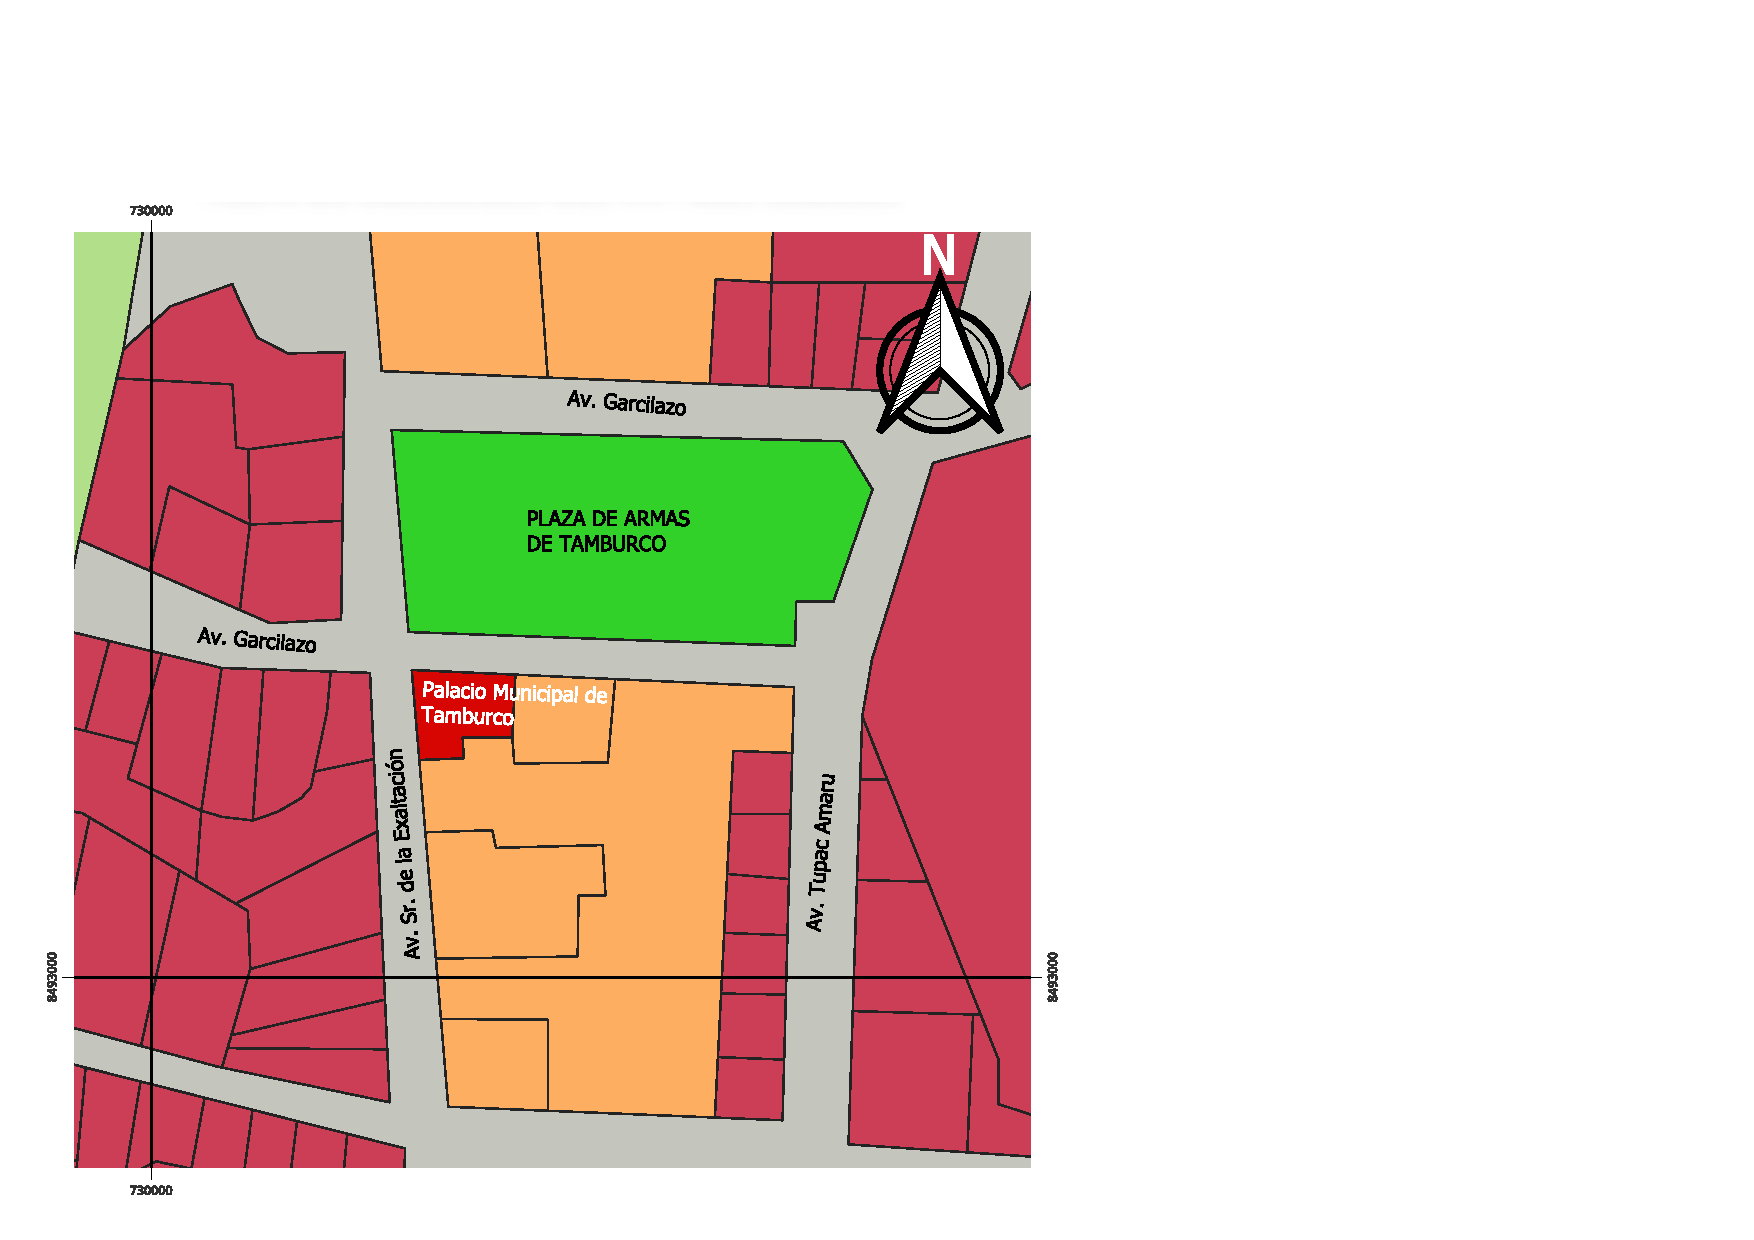
\includegraphics[width=0.8\textwidth]{2.0.pdf}\\
	\caption[Mapa de ubicación del Palacio Municipal]{Ubicación de la Municipalidad Distrital de Tamburco}
	\label{map_ubic}
\end{figure}
\section{Nombre del Representante Legal:}
\noindent Raúl Silva Campos\\
\textbf{Alcalde de la Municipalidad Distrital de Tamburco}

\section{Nombre del Jefe Inmediato:}
\noindent Ing. Ricardo Hemrich Pinto Yupanqui, Sub Gerente de Obras y Desarrollo Urbano y Rural.\\

\section{Teléfonos:}
\begin{itemize}
	\item Jefe Inmediato: 952717755
	\item Representante Legal:
\end{itemize}

\vspace{3mm}
\begin{figure}[h!]
	\captionsetup{width=0.8\textwidth}
	\centering
	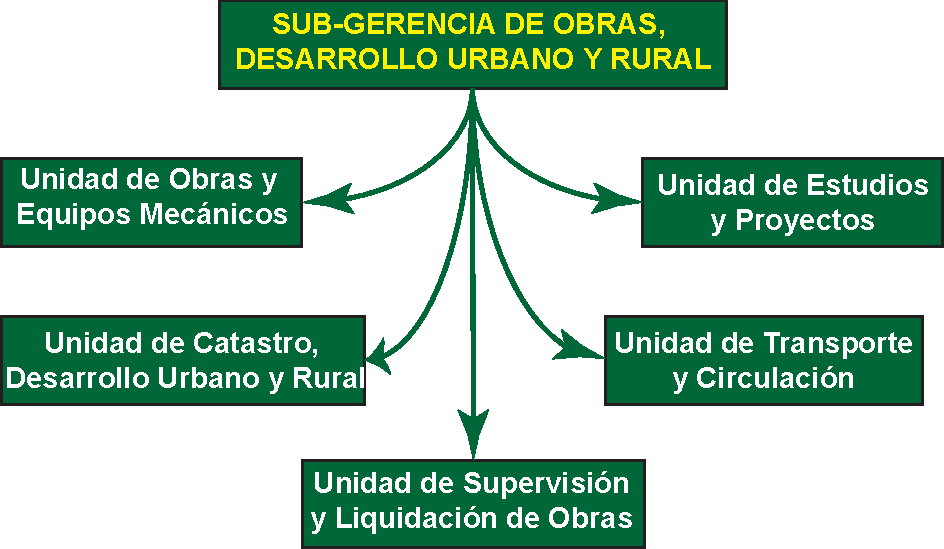
\includegraphics[width=0.8\textwidth]{2.5.pdf}
	\caption{Distribución en unidades de la SGODUR}
	\label{fig:2.5}
\end{figure}
\newpage
\begin{figure}[H]
	\centering
	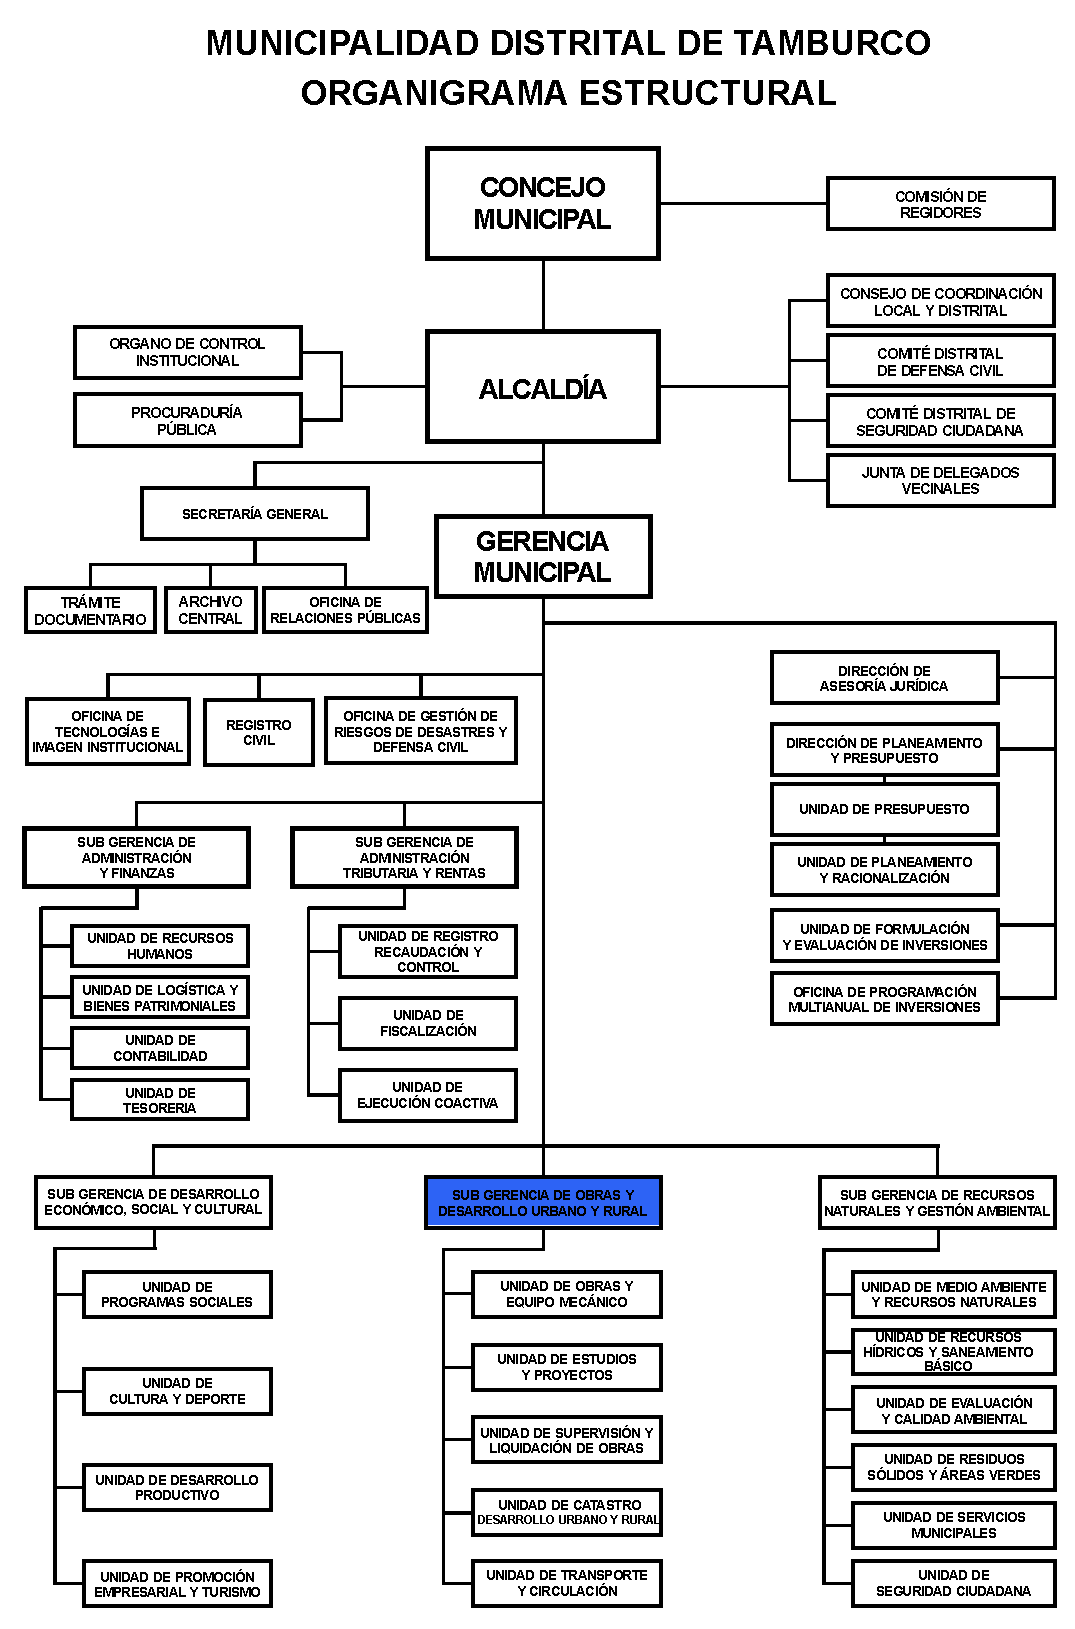
\includegraphics[height=24cm]{2.4.pdf}
	\caption[Organigrama de la Municipalidad Distrital de Tamburco]{Fuente:Municipalidad Distrital de Tamburco}
	\label{fig:organigrama-tamburco}
\end{figure}